% Compile with: pdflatex cs173_notes.tex (twice for ToC)
% Requires: amsmath, amssymb, amsthm, stmaryrd, mathtools, xcolor, mdframed,
%           enumitem, hyperref, pagecolor, microtype, tikz, titlesec
\documentclass[11pt]{article}
\usepackage[margin=1in]{geometry}
\usepackage{amsmath, amssymb, amsthm}
\usepackage{stmaryrd}
\usepackage{mathtools}
\usepackage{xcolor}
\usepackage{mdframed}
\usepackage{enumitem}
\usepackage{hyperref}
\usepackage{pagecolor}
\usepackage[expansion=false]{microtype}
\usepackage{tikz}
\usepackage{titlesec}
\usepackage{fancyhdr}
\usepackage{tocloft}
\usetikzlibrary{arrows.meta, positioning, shapes.geometric}

% Fix headheight to suppress fancyhdr warnings
\setlength{\headheight}{14pt}

% Tighter TOC spacing to keep contents on a single page
\setlength{\cftbeforepartskip}{4pt}
\setlength{\cftbeforesecskip}{1pt}
\setlength{\cftbeforesubsecskip}{0pt}

% ── Colour palette ───────────────────────────────────────────────
\definecolor{cream}{HTML}{FFFDF5}
\definecolor{defblue}{HTML}{1A4A7A}
\definecolor{thmgreen}{HTML}{1A5C3A}
\definecolor{warnAmber}{HTML}{7A4A00}
\definecolor{dangerRed}{HTML}{7A1A1A}
\definecolor{boxbluebg}{HTML}{EBF3FB}
\definecolor{boxgreenbg}{HTML}{EBF7EF}
\definecolor{boxamberbg}{HTML}{FDF5E6}
\definecolor{boxredbg}{HTML}{FBEBEB}
\pagecolor{cream}

% ── Hyperlink colours (must come after colour definitions) ──────
\hypersetup{
  colorlinks=true,
  linkcolor=black,
  urlcolor=defblue,
  citecolor=black
}

% ── Part / section styling ───────────────────────────────────────
\titleformat{\part}[display]
  {\normalfont\Huge\bfseries}
  {\filcenter\Large Part \thepart}
  {12pt}
  {\filcenter}
\titleformat{\section}
  {\normalfont\Large\bfseries}
  {\thesection}{1em}{}
\titleformat{\subsection}
  {\normalfont\large\bfseries}
  {\thesubsection}{1em}{}

% ── Header / footer ──────────────────────────────────────────────
\pagestyle{fancy}
\fancyhf{}
\fancyhead[L]{\small\color{gray} CS 173 --- Discrete Structures}
\fancyhead[R]{\small\color{gray} Mohammed Al Salhi}
\fancyfoot[C]{\thepage}
\renewcommand{\headrulewidth}{0.4pt}
\renewcommand{\headrule}{\color{gray}\hrule width\textwidth}

% ── Theorem styles ───────────────────────────────────────────────
\newtheoremstyle{defstyle}    {8pt}{8pt}{\normalfont}{0pt}{\bfseries\color{defblue}}  {.}{0.5em}{}
\newtheoremstyle{thmstyle}    {8pt}{8pt}{\normalfont}{0pt}{\bfseries\color{thmgreen}} {.}{0.5em}{}
\newtheoremstyle{notstyle}    {8pt}{8pt}{\normalfont}{0pt}{\bfseries\color{warnAmber}}{.}{0.5em}{}
\newtheoremstyle{cautionstyle}{8pt}{8pt}{\normalfont}{0pt}{\bfseries\color{dangerRed}}{.}{0.5em}{}

\theoremstyle{defstyle}
\newtheorem{definition}{Definition}[section]

\theoremstyle{thmstyle}
\newtheorem{theorem}{Theorem}[section]
\newtheorem{corollary}[theorem]{Corollary}
\newtheorem{lemma}[theorem]{Lemma}
\newtheorem{proposition}[theorem]{Proposition}

\theoremstyle{notstyle}
\newtheorem*{remark}{Remark}
\newtheorem*{example}{Example}

\theoremstyle{cautionstyle}
\newtheorem*{caution}{Caution}

% ── Framed boxes ─────────────────────────────────────────────────
\newmdenv[
  backgroundcolor=boxbluebg, linecolor=defblue, linewidth=2pt,
  topline=false, rightline=false, bottomline=false,
  innerleftmargin=10pt, innerrightmargin=10pt,
  innertopmargin=6pt, innerbottommargin=6pt,
  skipabove=8pt, skipbelow=8pt
]{defbox}

\newmdenv[
  backgroundcolor=boxgreenbg, linecolor=thmgreen, linewidth=2pt,
  topline=false, rightline=false, bottomline=false,
  innerleftmargin=10pt, innerrightmargin=10pt,
  innertopmargin=6pt, innerbottommargin=6pt,
  skipabove=8pt, skipbelow=8pt
]{thmbox}

\newmdenv[
  backgroundcolor=boxamberbg, linecolor=warnAmber, linewidth=2pt,
  topline=false, rightline=false, bottomline=false,
  innerleftmargin=10pt, innerrightmargin=10pt,
  innertopmargin=6pt, innerbottommargin=6pt,
  skipabove=8pt, skipbelow=8pt
]{notebox}

\newmdenv[
  backgroundcolor=boxredbg, linecolor=dangerRed, linewidth=2pt,
  topline=false, rightline=false, bottomline=false,
  innerleftmargin=10pt, innerrightmargin=10pt,
  innertopmargin=6pt, innerbottommargin=6pt,
  skipabove=8pt, skipbelow=8pt
]{cautionbox}

% ── Macros ───────────────────────────────────────────────────────
\newcommand{\Z}{\mathbb{Z}}
\newcommand{\N}{\mathbb{N}}
\newcommand{\R}{\mathbb{R}}
\newcommand{\Q}{\mathbb{Q}}
\newcommand{\Zn}{\mathbb{Z}_n}
\newcommand{\Np}{\mathbb{N}^{+}}
\newcommand{\modn}{\pmod{n}}
\newcommand{\id}{\mathrm{id}}
\newcommand{\card}[1]{\lvert #1 \rvert}
\newcommand{\Pow}{\mathcal{P}}

\begin{document}

% ════════════════════════════════════════════════════════════════
% TITLE PAGE
% ════════════════════════════════════════════════════════════════
\thispagestyle{empty}
\begin{center}
  \vspace*{2cm}
  {\Huge\bfseries CS 173 --- Discrete Structures}\\[10pt]
  {\Large Lectures 24--35: A Unified Treatment}\\[6pt]
  {\large Modular Arithmetic, Functions, Cardinality,\\and Graph Theory}\\[2cm]

  \begin{minipage}{0.8\textwidth}
  \centering\itshape\small\color{gray}
  These notes consolidate Lectures 24 and 26--35 into a single coherent
  arc: from equivalence relations (modular congruence) through functions
  and cardinality to applications in graph theory.  Each part builds
  directly on the previous one; reading in order is recommended.
  \end{minipage}\\[2cm]

  Mohammed Al Salhi\\[2pt]
  {\small\color{gray} University of Illinois at Urbana-Champaign}\\[2pt]
  {\small\color{gray} Spring 2026}
\end{center}
\vfill

\newpage
\tableofcontents
\newpage

% ════════════════════════════════════════════════════════════════
% PART I --- MODULAR ARITHMETIC
% ════════════════════════════════════════════════════════════════
\part{Modular Arithmetic}

This part introduces the first non-trivial example of an equivalence
relation we'll meet in the course: \emph{congruence modulo $n$}.  The
algebraic structure $(\Zn, +, \cdot)$ that emerges is a useful object
in its own right, and it foreshadows a recurring theme --- defining
``equality up to'' a structural relation.

% ----------------------------------------------------------------
\section{Congruence modulo \texorpdfstring{$n$}{n}}

\begin{defbox}
\begin{definition}[Congruence modulo $n$]
For $x, y \in \Z$ and $n \in \Np$, $x$ is \emph{congruent to $y$ modulo
$n$}, written $x \equiv y \modn$, iff $n \mid (x-y)$.
\end{definition}
\end{defbox}

\begin{notebox}
\begin{remark}
Read $\equiv$ as a structured equality: rather than asking whether two
integers are identical, we ask whether they leave the same remainder when
divided by $n$.
\end{remark}
\end{notebox}

\begin{thmbox}
\begin{theorem}[$\equiv \modn$ is an equivalence relation]
For all $n \in \Np$:
\begin{enumerate}[label=\textnormal{(\roman*)}, leftmargin=2em, itemsep=2pt]
  \item \textbf{Reflexive}: $x \equiv x \modn$ since $n \mid 0$.
  \item \textbf{Symmetric}: $x \equiv y \Rightarrow y \equiv x$, since
        $n \mid (x-y) \Rightarrow n \mid -(x-y)$.
  \item \textbf{Transitive}: $x \equiv y$ and $y \equiv z$ imply
        $x \equiv z$, since $n \mid (x-y) + (y-z) = x-z$.
\end{enumerate}
\end{theorem}
\end{thmbox}

% ----------------------------------------------------------------
\section{Compatibility with arithmetic}

\begin{thmbox}
\begin{theorem}[Compatibility]
For all $n \in \Np$ and all $x, y, z \in \Z$, if $x \equiv y \modn$ then
\[
  x + z \equiv y + z \modn
  \qquad\text{and}\qquad
  x \cdot z \equiv y \cdot z \modn.
\]
\end{theorem}
\end{thmbox}

\begin{thmbox}
\begin{theorem}[Cancellation]
\textbf{Additive cancellation} holds unconditionally:
\[
  x + z \equiv y + z \modn \;\Rightarrow\; x \equiv y \modn.
\]
\textbf{Multiplicative cancellation} holds only when $\gcd(z, n) = 1$:
\[
  x \cdot z \equiv y \cdot z \modn \;\wedge\; \gcd(z,n) = 1
  \;\Rightarrow\; x \equiv y \modn.
\]
\end{theorem}
\end{thmbox}

\begin{cautionbox}
\begin{caution}[Multiplicative cancellation can fail]
Without the coprimality hypothesis, multiplicative cancellation breaks.
E.g.\ in $\Z_6$: $2 \cdot 2 = 4$ and $2 \cdot 5 = 10 \equiv 4$, so
$2 \cdot 2 \equiv 2 \cdot 5 \pmod 6$, but $2 \not\equiv 5 \pmod 6$.  The
issue: $\gcd(2, 6) = 2 \neq 1$.
\end{caution}
\end{cautionbox}

% ----------------------------------------------------------------
\section{The ring \texorpdfstring{$\Zn$}{Z\_n}}

\begin{defbox}
\begin{definition}[Integers modulo $n$]
For $n \in \Np$, define $\Zn := \{0, 1, 2, \ldots, n-1\}$, the set of
\emph{residues} modulo $n$.  Define modular operations on $\Zn$ by
\[
  a \oplus b := (a + b) \bmod n,
  \qquad
  a \otimes b := (a \cdot b) \bmod n.
\]
\end{definition}
\end{defbox}

\begin{notebox}
\begin{example}[Working in $\Z_6$]
The additive inverses pair up:
\[
  1+5 \equiv 0,\quad 2+4 \equiv 0,\quad 3+3 \equiv 0 \pmod 6.
\]
Each pair $(a, 6-a)$ sums to $0$.
\end{example}
\end{notebox}

\begin{thmbox}
\begin{theorem}[Algebraic properties of $\Zn$]
$(\Zn, \oplus, \otimes)$ is a \emph{commutative ring}: $\oplus$ and
$\otimes$ are commutative and associative, $\otimes$ distributes over
$\oplus$, $0$ is the additive identity, $1$ is the multiplicative
identity, and every $a \in \Zn$ has additive inverse $n - a$.
\end{theorem}
\end{thmbox}

\begin{cautionbox}
\begin{caution}[Multiplicative inverses are not guaranteed]
$a \in \Zn$ has a multiplicative inverse iff $\gcd(a, n) = 1$.  When $n$
is prime, every nonzero element is invertible and $\Zn$ is a \emph{field}.
\end{caution}
\end{cautionbox}

\begin{notebox}
\begin{remark}[Looking ahead]
The ring properties of $\Zn$ underpin the solution of linear congruences
$ax \equiv b \modn$ via the extended Euclidean algorithm.  The deeper
takeaway, though, is the pattern: an equivalence relation on $\Z$
produces a quotient set $\Zn$ that inherits a coherent algebraic
structure.  This pattern reappears throughout discrete mathematics.
\end{remark}
\end{notebox}

\newpage

% ════════════════════════════════════════════════════════════════
% PART II --- FUNCTIONS
% ════════════════════════════════════════════════════════════════
\part{Functions}

We now turn to the language of functions.  Three classes of functions
--- injections, surjections, and bijections --- form the bedrock for
everything that follows.  In Part III we use them to compare the sizes
of sets, finite or infinite.

% ----------------------------------------------------------------
\section{Injections, surjections, bijections}

Throughout this section let $A, B$ be sets and $f \colon A \to B$ a function.

\begin{defbox}
\begin{definition}[Injection / one-to-one]
$f$ is \emph{injective} iff distinct inputs produce distinct outputs:
\[
  \forall a_1, a_2 \in A,\;\; f(a_1) = f(a_2) \;\Rightarrow\; a_1 = a_2.
\]
Equivalently (by contraposition), $a_1 \neq a_2 \Rightarrow f(a_1) \neq f(a_2)$.
\end{definition}
\end{defbox}

\begin{defbox}
\begin{definition}[Surjection / onto]
$f$ is \emph{surjective} iff every element of $B$ is hit:
\[
  \forall y \in B,\; \exists x \in A,\; f(x) = y.
\]
\end{definition}
\end{defbox}

\begin{defbox}
\begin{definition}[Bijection]
$f$ is a \emph{bijection} iff it is both injective and surjective.
\end{definition}
\end{defbox}

\subsection{Diagrammatic intuition}

\begin{center}
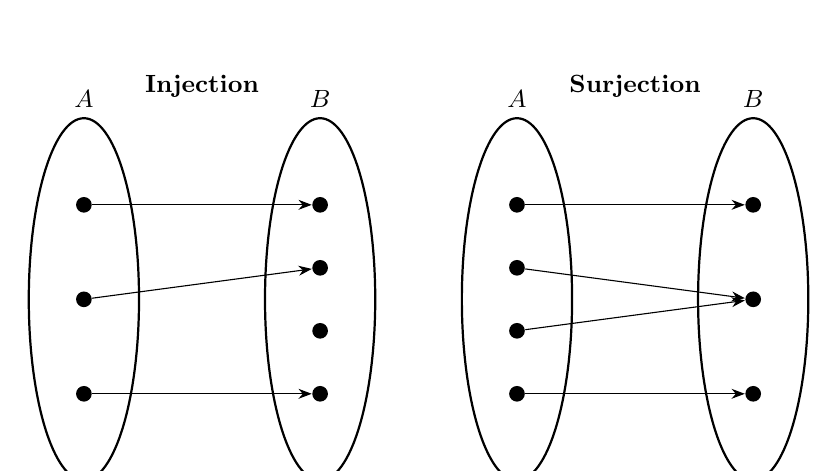
\begin{tikzpicture}[
    every node/.style={font=\small},
    dot/.style={circle, fill, inner sep=2pt},
    >=Stealth
  ]
  % Injection
  \begin{scope}[xshift=0cm]
    \node[font=\bfseries\small] at (1.5, 3.7) {Injection};
    \draw[thick] (0, 1) ellipse (0.7cm and 2.3cm);
    \node at (0, 3.55) {$A$};
    \node[dot] (a1) at (0,  2.2) {};
    \node[dot] (a2) at (0,  1.0) {};
    \node[dot] (a3) at (0, -0.2) {};
    \draw[thick] (3, 1) ellipse (0.7cm and 2.3cm);
    \node at (3, 3.55) {$B$};
    \node[dot] (b1) at (3,  2.2) {};
    \node[dot] (b2) at (3,  1.4) {};
    \node[dot] (b3) at (3,  0.6) {};
    \node[dot] (b4) at (3, -0.2) {};
    \draw[->] (a1) -- (b1);
    \draw[->] (a2) -- (b2);
    \draw[->] (a3) -- (b4);
  \end{scope}
  % Surjection
  \begin{scope}[xshift=5.5cm]
    \node[font=\bfseries\small] at (1.5, 3.7) {Surjection};
    \draw[thick] (0, 1) ellipse (0.7cm and 2.3cm);
    \node at (0, 3.55) {$A$};
    \node[dot] (c1) at (0,  2.2) {};
    \node[dot] (c2) at (0,  1.4) {};
    \node[dot] (c3) at (0,  0.6) {};
    \node[dot] (c4) at (0, -0.2) {};
    \draw[thick] (3, 1) ellipse (0.7cm and 2.3cm);
    \node at (3, 3.55) {$B$};
    \node[dot] (d1) at (3,  2.2) {};
    \node[dot] (d2) at (3,  1.0) {};
    \node[dot] (d3) at (3, -0.2) {};
    \draw[->] (c1) -- (d1);
    \draw[->] (c2) -- (d2);
    \draw[->] (c3) -- (d2);
    \draw[->] (c4) -- (d3);
  \end{scope}
\end{tikzpicture}
\end{center}

\begin{center}
\renewcommand{\arraystretch}{1.5}
\begin{tabular}{|l|l|l|}
\hline
\textbf{Property} & \textbf{Injection} & \textbf{Surjection} \\
\hline
Statement       & $f(a_1)=f(a_2) \Rightarrow a_1=a_2$ & $\forall y \in B,\; \exists x \in A,\; f(x)=y$ \\
Constraint on   & inputs (domain $A$) & outputs (codomain $B$) \\
Violation       & two arrows into one dot in $B$ & a dot in $B$ with no arrow \\
\hline
\end{tabular}
\end{center}

% ----------------------------------------------------------------
\section{Inverses, monomorphisms, epimorphisms}

\begin{defbox}
\begin{definition}[Identity, left/right inverse]
The \emph{identity function} $\id_A \colon A \to A$ is $\id_A(a) = a$.
A function $g \colon B \to A$ is a \emph{left inverse} of $f \colon A \to B$
if $g \circ f = \id_A$, and a \emph{right inverse} if $f \circ g = \id_B$.
\end{definition}
\end{defbox}

\begin{defbox}
\begin{definition}[Mono / epi / iso]
Let $f \colon A \to B$.
\begin{itemize}[leftmargin=2em, itemsep=2pt]
  \item $f$ is a \emph{monomorphism} (or \emph{monic}) iff $f$ has a left inverse.
  \item $f$ is an \emph{epimorphism} (or \emph{epic}) iff $f$ has a right inverse.
  \item $f$ is an \emph{isomorphism} iff $f$ is both monic and epic.
\end{itemize}
\end{definition}
\end{defbox}

\begin{thmbox}
\begin{theorem}[Inverses from injections / surjections]
Let $f \colon A \to B$.
\begin{enumerate}[label=\textnormal{(\Roman*)}, leftmargin=2.5em, itemsep=2pt]
  \item If $f$ is injective and $A \neq \emptyset$, there exists a
        \emph{surjective} $g \colon B \to A$ with $g \circ f = \id_A$.
  \item If $f$ is surjective, there exists an \emph{injective}
        $g \colon B \to A$ with $f \circ g = \id_B$.
\end{enumerate}
\end{theorem}
\end{thmbox}

\begin{cautionbox}
\begin{caution}[Empty-domain corner case]
Part~(I) fails when $A = \emptyset$ and $B \neq \emptyset$: the empty
function is vacuously injective, but no $g \colon B \to \emptyset$ exists.
\end{caution}
\end{cautionbox}

\begin{thmbox}
\begin{corollary}[Two-sided inverse of a bijection]
If $f \colon A \to B$ is a bijection, there exists a \emph{unique}
bijection $g \colon B \to A$ satisfying both $g \circ f = \id_A$ and
$f \circ g = \id_B$.  This $g$ is denoted $f^{-1}$.
\end{corollary}
\end{thmbox}

\begin{notebox}
\begin{remark}
Uniqueness fails on one side alone --- a non-surjective injection has
many left inverses (any preimage choice on $B \setminus f(A)$).
Two-sidedness is what pins $g$ down.
\end{remark}
\end{notebox}

\subsection{Cancellation characterisation}

The same three notions can be characterised \emph{purely by composition},
without referring to elements.

\begin{thmbox}
\begin{theorem}[Cancellation forms]
Let $f \colon A \to B$.
\begin{enumerate}[label=\textnormal{(\arabic*)}, leftmargin=2em, itemsep=2pt]
  \item $f$ is injective $\iff$ $\forall W,\, h_1, h_2 \colon W \to A,\;
        f \circ h_1 = f \circ h_2 \Rightarrow h_1 = h_2$.
  \item $f$ is surjective $\iff$ $\forall Z,\, k_1, k_2 \colon B \to Z,\;
        k_1 \circ f = k_2 \circ f \Rightarrow k_1 = k_2$.
  \item $f$ is a bijection $\iff$ $f$ has a two-sided inverse.
\end{enumerate}
\end{theorem}
\end{thmbox}

\begin{notebox}
\begin{remark}[Why this matters]
The ``element-level'' definitions look inside $A$ and $B$; the
cancellation forms only mention compositions.  This generalises to
settings where objects don't have ``elements'' --- the entry point to
category theory.
\end{remark}
\end{notebox}

\newpage

% ════════════════════════════════════════════════════════════════
% PART III --- CARDINALITY
% ════════════════════════════════════════════════════════════════
\part{Cardinality}

We use injections and surjections to compare set sizes --- a definition
that works equally well for finite and infinite sets.

% ----------------------------------------------------------------
\section{Comparing cardinalities}

\begin{defbox}
\begin{definition}[Cardinality comparisons]
For sets $A, B$:
\begin{itemize}[leftmargin=2em, itemsep=2pt]
  \item $\card{A} \leq \card{B} \iff \exists f \colon A \to B$ injective.
  \item If $B \neq \emptyset$:
        $\card{A} \geq \card{B} \iff \exists f \colon A \to B$ surjective.\\
        \emph{Empty target convention:} $\card{A} \geq \card{\emptyset}$
        for all $A$.
  \item $\card{A} = \card{B} \iff \exists f \colon A \to B$ a bijection
        $\iff \card{A} \leq \card{B}$ and $\card{A} \geq \card{B}$.
\end{itemize}
\end{definition}
\end{defbox}

\begin{notebox}
\begin{remark}[Why the asymmetry]
An injection $A \hookrightarrow B$ ``fits'' all of $A$ into $B$ without
collisions, so $B$ must be at least as large.  A surjection
$A \twoheadrightarrow B$ ``covers'' all of $B$, so $A$ must be at least
as large.  The empty target is a degenerate case: no surjection
$A \to \emptyset$ exists when $A \neq \emptyset$, so we patch the
definition by fiat.
\end{remark}
\end{notebox}

% ----------------------------------------------------------------
\section{Order-theoretic properties}

\begin{thmbox}
\begin{theorem}[Order properties of $\leq$]
For all sets $A, B, C$:
\begin{enumerate}[label=\textnormal{(\roman*)}, leftmargin=2em, itemsep=2pt]
  \item \textbf{Reflexive}: $\card{A} = \card{A}$ \;(witnessed by $\id_A$).
  \item \textbf{Duality}: $\card{A} \leq \card{B} \iff \card{B} \geq \card{A}$.
  \item \textbf{Transitive}: $\card{A} \leq \card{B}$ and $\card{B} \leq \card{C}$
        $\Rightarrow$ $\card{A} \leq \card{C}$ \;(witnessed by composition).
  \item \textbf{Antisymmetric (Cantor--Schröder--Bernstein)}:
        $\card{A} \leq \card{B}$ and $\card{A} \geq \card{B}$
        $\Rightarrow$ $\card{A} = \card{B}$.
  \item \textbf{Trichotomy} (Axiom 7, equivalent to AC):
        $\card{A} \leq \card{B}$ or $\card{A} \geq \card{B}$.
\end{enumerate}
\end{theorem}
\end{thmbox}

\begin{notebox}
\begin{remark}[CSB is the deep part]
For finite sets, antisymmetry follows from counting.  For infinite sets,
it requires \emph{constructing} a bijection from two given injections ---
the content of CSB.  Trichotomy is independent of ZF, equivalent to AC.
\end{remark}
\end{notebox}

\begin{defbox}
\begin{definition}[Strict cardinality]
$\card{A} < \card{B}$ iff there is an injection $A \to B$ but no
surjection $A \to B$.  Symmetrically, $\card{A} > \card{B}$ iff there is
a surjection $A \to B$ but no injection $A \to B$.
\end{definition}
\end{defbox}

\begin{notebox}
\begin{remark}
Each strict definition pairs an existential witness with a universal
failure.  The universal clause cannot be skipped --- a single
non-surjective function (e.g.\ a constant) proves nothing on its own.
\end{remark}
\end{notebox}

% ----------------------------------------------------------------
\section{Finite sets}

\begin{defbox}
\begin{definition}[Finite set, cardinality of a finite set]
Identify $n \in \N$ with the set $\{0, 1, \ldots, n-1\}$.
A set $X$ is \emph{finite} iff $\card{X} = \card{n}$ for some $n \in \N$.
The unique such $n$ is then called $\card{X}$.
\end{definition}
\end{defbox}

\begin{notebox}
\begin{remark}[Why $n$ is unique]
Distinct naturals $m \neq n$ admit no bijection between them, so
antisymmetry forces the matching $n$ to be unique.
\end{remark}
\end{notebox}

\subsection{Counting laws}

\begin{thmbox}
\begin{theorem}[Counting laws on finite sets]
If $X, Y$ are finite then so are $X \cap Y$, $X \cup Y$, $X \setminus Y$,
and $X \times Y$.  Moreover:
\begin{enumerate}[label=\textnormal{(\roman*)}, leftmargin=2em, itemsep=2pt]
  \item \emph{Subset subtraction:} If $Y \subseteq X$, then
        $\card{X \setminus Y} = \card{X} - \card{Y}$.
  \item \emph{General subtraction:}
        $\card{X \setminus Y} = \card{X} - \card{X \cap Y}$.
  \item \emph{Inclusion--exclusion (two-set):}
        $\card{X \cup Y} = \card{X} + \card{Y} - \card{X \cap Y}$.
  \item \emph{Union bound:}
        $\bigl|\bigcup_{i=1}^n A_i\bigr| \leq \sum_{i=1}^n \card{A_i}$,
        with equality iff the $A_i$ are pairwise disjoint.
  \item \emph{Product:} $\card{X \times Y} = \card{X} \cdot \card{Y}$.
\end{enumerate}
\end{theorem}
\end{thmbox}

\subsection{Single-element removal}

The following lemma is the key induction step in many counting
arguments; the proof is included because the technique --- gap-closing
relabelling --- recurs throughout the course.

\begin{thmbox}
\begin{lemma}[Removing one element]
For any finite set $X$ and $a \in X$, $\card{X \setminus \{a\}} = \card{X} - 1$.
\end{lemma}
\begin{proof}
Let $\card{X} = n$, fix a bijection $f \colon X \to n = \{0, \ldots, n-1\}$.
Define $g \colon X \setminus \{a\} \to n - 1$ by
\[
  g(b) = \begin{cases} f(b) & \text{if } f(b) < f(a), \\
                       f(b) - 1 & \text{if } f(b) > f(a). \end{cases}
\]
The two cases are mutually exclusive because $b \neq a$ and $f$ is
injective.  We verify $g$ is a bijection.

\smallskip
\textit{Injective.}\;
Suppose $g(b_1) = g(b_2)$.  If $f(b_1) < f(a)$ and $f(b_2) > f(a)$, then
$g(b_1) = f(b_1) < f(a)$ but $g(b_2) = f(b_2) - 1 \geq f(a)$, a
contradiction.  So $f(b_1)$ and $f(b_2)$ lie on the same side of $f(a)$,
in which case $g(b_1) = g(b_2)$ forces $f(b_1) = f(b_2)$, hence $b_1 = b_2$
by injectivity of $f$.

\smallskip
\textit{Surjective.}\;
Let $y \in n - 1$.  If $y < f(a)$, then since $f$ is surjective there is
$b \in X$ with $f(b) = y$; we have $b \neq a$ (else $y = f(a)$), so
$g(b) = f(b) = y$.  If $y \geq f(a)$, then $y + 1 \in n$ and there is
$b \in X$ with $f(b) = y+1 > f(a)$; again $b \neq a$, and
$g(b) = f(b) - 1 = y$.

\smallskip
Hence $g$ is a bijection, so $\card{X \setminus \{a\}} = n - 1$.
\end{proof}
\end{thmbox}

% ----------------------------------------------------------------
\section{Pigeonhole principle}

\begin{thmbox}
\begin{theorem}[Pigeonhole]
Let $A, B$ be sets.
\begin{enumerate}[label=\textnormal{(\roman*)}, leftmargin=2em, itemsep=2pt]
  \item $\card{A} > \card{B} \;\Rightarrow\;$ no $f \colon A \to B$ is injective.
  \item $\card{A} < \card{B} \;\Rightarrow\;$ no $f \colon A \to B$ is surjective.
\end{enumerate}
\end{theorem}
\end{thmbox}

\begin{thmbox}
\begin{theorem}[Quantitative pigeonhole]
Let $\card{A} = n \in \Np$, $\card{B} = k \in \Np$, $f \colon A \to B$.
Then some fibre is large:
\[
  \exists b \in B,\;\; \bigl|\{a \in A \mid f(a) = b\}\bigr|
    \;\geq\; \left\lceil \tfrac{n}{k} \right\rceil.
\]
\end{theorem}
\end{thmbox}

\begin{notebox}
\begin{remark}[Why the bound]
If every fibre had size $< \lceil n/k \rceil$, the total
$\sum_b \card{f^{-1}(\{b\})}$ would be at most
$k(\lceil n/k \rceil - 1) < n$, contradicting that the fibres partition
$A$ and so sum to $\card{A} = n$.
\end{remark}
\end{notebox}

\begin{thmbox}
\begin{proposition}[Finite shortcut]
For \emph{finite} $A, B$:
\begin{itemize}[leftmargin=2em, itemsep=2pt]
  \item An injective non-surjection $A \to B$ witnesses $\card{A} < \card{B}$.
  \item A surjective non-injection $A \to B$ witnesses $\card{A} > \card{B}$.
\end{itemize}
\end{proposition}
\end{thmbox}

\begin{cautionbox}
\begin{caution}[Infinite sets break the shortcut]
Take $f \colon \N \to \N,\; n \mapsto 2n$: injective, not surjective, yet
$\card{\N} = \card{\N}$.  For strict comparisons in the infinite case, the
universal clause must be proved directly --- the job of Cantor's diagonal.
\end{caution}
\end{cautionbox}

% ----------------------------------------------------------------
\section{Infinite sets}

\begin{defbox}
\begin{definition}[Infinite, Dedekind infinite]
A set $X$ is \emph{infinite} iff $X$ is not finite, i.e.\
$\forall n \in \N,\; \card{X} \neq \card{n}$.

$X$ is \emph{Dedekind infinite} iff some \emph{proper} subset
$Y \subsetneq X$ satisfies $\card{Y} = \card{X}$.
\end{definition}
\end{defbox}

\begin{thmbox}
\begin{theorem}[Equivalence]
$X$ is infinite $\iff$ $X$ is Dedekind infinite.
\end{theorem}
\end{thmbox}

\begin{notebox}
\begin{remark}[Status of the proof]
The $(\Leftarrow)$ direction is straightforward.  The $(\Rightarrow)$
direction requires the Axiom of Choice in full generality.  The two
constructions below witness the Dedekind side concretely for $\N$.
\end{remark}
\end{notebox}

\subsection{\texorpdfstring{$\N$}{N} is genuinely infinite}

\begin{thmbox}
\begin{theorem}
$\N$ is infinite.
\end{theorem}
\begin{proof}
Suppose, for contradiction, that there is a bijection $f \colon n \to \N$
for some $n \in \N$.  Let $S = \sum_{i=0}^{n-1} f(i) \in \N$.  Each $f(i)$
is non-negative, so $f(i) \leq S < S + 1$ for every $i$.  By
surjectivity of $f$, some $x \in n$ satisfies $f(x) = S + 1$,
contradicting $f(x) \leq S$.
\end{proof}
\end{thmbox}

\subsection{Bijections between countably infinite sets}

\begin{thmbox}
\begin{theorem}[Same-size infinities]
$\card{\N} = \card{\Np} = \card{\Z} = \card{E} = \card{\N \times \N}$,
where $E$ is the set of even integers.
\end{theorem}
\begin{proof}[Sketch]
Each equality is witnessed by an explicit bijection; combined with the
identity injections in the obvious directions, Cantor--Schröder--Bernstein
finishes the harder cases.

\smallskip
\noindent$\card{\N} = \card{\Np}$:\; $n \mapsto n + 1$.

\smallskip
\noindent$\card{\Z} = \card{\N}$:\; interleave non-negatives and negatives,
\[
  f(x) = \begin{cases} 2x & x \geq 0, \\ -2x - 1 & x < 0. \end{cases}
\]
First several values: $0 \mapsto 0,\; -1 \mapsto 1,\; 1 \mapsto 2,\;
-2 \mapsto 3,\; 2 \mapsto 4, \ldots$

\smallskip
\noindent$\card{\N} = \card{E}$:\; analogously, $f \colon \N \to E$ given by
$f(n) = n$ if $n$ even, $f(n) = -n - 1$ if $n$ odd.

\smallskip
\noindent$\card{\N \times \N} = \card{\N}$:\; the inclusion $n \mapsto (0, n)$
gives one injection.  The encoding $(x, y) \mapsto 2^x \cdot 3^y$ gives
the other --- injective by unique prime factorisation, since $2$ and $3$
are distinct primes.  CSB closes the argument.
\end{proof}
\end{thmbox}

\begin{cautionbox}
\begin{caution}[Bad encodings]
Tempting alternatives like $(x,y) \mapsto 2^x + 3^y$ or
$(x,y) \mapsto x + y$ are \emph{not} injective.  Multiplicativity together
with distinct prime bases is exactly what unique factorisation needs.
\end{caution}
\end{cautionbox}

\subsection{Hilbert's hotel}

The bijections above admit a vivid retelling.  Imagine a hotel with rooms
labelled $\Np$, every room occupied by guest $G_n$.

\begin{center}
\renewcommand{\arraystretch}{1.5}
\begin{tabular}{|l|l|l|}
\hline
\textbf{Scenario} & \textbf{Reassignment} & \textbf{Underlying bijection} \\
\hline
$1$ new guest      & $G_n \to$ room $n+1$
                   & $n \mapsto n+1$ \\
Bus of $\Np$ guests & $G_n \to$ room $2n$,\; $H_k \to$ room $2k-1$
                   & $\Np \sqcup \Np \to \Np$ \\
\hline
\end{tabular}
\end{center}

\begin{cautionbox}
\begin{caution}[Simultaneous, not sequential]
Hilbert's reassignment is a single global act, not a process.  There is no
``last'' guest to move, so the bijection cannot be built one step at a time.
\end{caution}
\end{cautionbox}

% ----------------------------------------------------------------
\section{Cantor's theorem and the hierarchy of infinities}

So far every countably infinite set we've seen has $\card{\N}$.  Cantor
shows the power set genuinely grows the cardinality.

\begin{thmbox}
\begin{theorem}[Cantor]
$\card{X} < \card{\Pow(X)}$ for every set $X$.
\end{theorem}
\begin{proof}[Diagonal argument]
The map $x \mapsto \{x\}$ is an injection $X \to \Pow(X)$, so
$\card{X} \leq \card{\Pow(X)}$.  For the strict inequality, we show no
$\varphi \colon X \to \Pow(X)$ is surjective.

Define the \emph{anti-diagonal set}
\(
  \Delta = \{x \in X \mid x \notin \varphi(x)\} \in \Pow(X).
\)
Suppose $\varphi$ were surjective.  Then $\varphi(\delta) = \Delta$ for
some $\delta \in X$, and the biconditional
\[
  \delta \in \Delta
  \iff \delta \notin \varphi(\delta)
  \iff \delta \notin \Delta
\]
is a contradiction.  So $\varphi$ is not surjective.
\end{proof}
\end{thmbox}

\begin{notebox}
\begin{remark}[Connections]
The same self-referential trick produces \emph{Russell's paradox} (let
$X$ be ``the set of all sets'', $\varphi$ the identity).  The contradiction
in Cantor's proof becomes a hard contradiction in naive set theory, which
is why ZFC excludes a universal set.

The diagonal name comes from imagining $\varphi$ as an infinite table:
row $x$, column $y$ records whether $y \in \varphi(x)$.  $\Delta$ is built
by walking down the diagonal and \emph{flipping} each entry, so it
disagrees with every row.
\end{remark}
\end{notebox}

\begin{notebox}
\begin{remark}[The hierarchy of infinities]
Iterating $\Pow$ gives a strictly increasing chain of cardinalities:
\[
  \card{\N} \;<\; \card{\Pow(\N)} \;<\; \card{\Pow(\Pow(\N))} \;<\; \cdots
\]
The first jump is the canonical leap from countable to uncountable:
$\card{\Pow(\N)} = \card{\R}$.
\end{remark}
\end{notebox}

\newpage

% ════════════════════════════════════════════════════════════════
% PART IV --- APPLICATIONS
% ════════════════════════════════════════════════════════════════
\part{Applications}

The cardinality machinery now pays off.  In \S\ref{sec:handshake} we use
pigeonhole to prove a classic combinatorial identity about parties; in
\S\ref{sec:graphs} we set up graph theory and prove the handshaking lemma
by induction.

% ----------------------------------------------------------------
\section{The handshake theorem}\label{sec:handshake}

\begin{thmbox}
\begin{theorem}[Handshake theorem]
Any room with at least two people contains two distinct people who have
shaken the same number of hands.
\end{theorem}
\end{thmbox}

\subsection*{Setup}

Fix $n \geq 2$.  Take $A = \{0, 1, \ldots, n-1\}$ for the set of people
($\card{A} = n$), and a symmetric handshake relation
$H \subseteq A \times A$.  Define
\[
  f \colon A \to B,\qquad f(p) = \bigl|\{a \in A \mid (p, a) \in H\}\bigr|,
\]
where $B \subseteq D = \{0, 1, \ldots, n-1\}$ is the set of \emph{actual}
handshake counts that occur.  The proof reduces to showing $\card{B} < \card{A}$,
then quoting pigeonhole.

\subsection*{The codomain bound}

\begin{thmbox}
\begin{lemma}[Codomain bound]
$\card{B} \leq n - 1$.
\end{lemma}
\begin{proof}
Either everyone has shaken $\geq 1$ hands or someone has shaken $0$.

\smallskip
\textit{Case 1: $0 \notin B$.}\;
Then $B \subseteq D \setminus \{0\}$, so $\card{B} \leq n - 1$.

\smallskip
\textit{Case 2: someone has shaken $0$ hands.}\;
Fix $p$ with $f(p) = 0$.  We show $n - 1 \notin B$ by contradiction.

Suppose $f(q) = n - 1$ for some $q$.  Then $q$ has shaken hands with
\emph{everyone else} --- the set
$\{a \in A \mid (q, a) \in H\} \subseteq A \setminus \{q\}$ has size
$n - 1 = \card{A \setminus \{q\}}$, so equality holds.  In particular,
$p \neq q$ (else $f(p) = f(q) = n - 1 \neq 0$), so $p \in A \setminus \{q\}$
and hence $(q, p) \in H$.  By symmetry $(p, q) \in H$, so
$f(p) \geq 1$, contradicting $f(p) = 0$.

So $n - 1 \notin B$, giving $\card{B} \leq n - 1$.
\end{proof}
\end{thmbox}

\begin{notebox}
\begin{remark}
The two cases knock out different elements of $D$: $0$ in Case 1,
$n - 1$ in Case 2.  The combined fact is that $\{0, n-1\}$ cannot both lie
in $B$ --- a universal hand-shaker and a hand-avoider can't coexist by
symmetry of $H$.
\end{remark}
\end{notebox}

\subsection*{Finishing with pigeonhole}

\begin{proof}[Proof of the handshake theorem]
$\card{B} < \card{A}$ by the lemma, so by pigeonhole $f$ is not
injective: there exist distinct $p_1, p_2 \in A$ with $f(p_1) = f(p_2)$.
\end{proof}

\begin{cautionbox}
\begin{caution}[$n \geq 2$ is needed]
With $n = 1$ the statement is vacuously \emph{false} (``two distinct
people'' don't exist).  The proof breaks too: Case~2 would need a single
person to satisfy $f(p) = 0$ \emph{and} have shaken everyone else's hand,
which is contradictory only because the universe ``everyone else'' is empty.
\end{caution}
\end{cautionbox}

\begin{notebox}
\begin{remark}[The template]
This is a template, not a one-off result.  Many ``in any group of $n$
objects, two must share a property'' proofs follow the same recipe:
build a counting function into a codomain that is provably one element
smaller than the domain, then quote pigeonhole.  The work is finding the
structural reason a particular value can't occur.
\end{remark}
\end{notebox}

% ----------------------------------------------------------------
\section{Graph theory}\label{sec:graphs}

\subsection{Graphs, neighbourhoods, degree}

\begin{defbox}
\begin{definition}[Graph]
A \emph{graph} $G$ is a pair $(V(G), E(G))$ where $V(G)$ is a finite set
of \emph{vertices} (or \emph{nodes}) and $E(G)$ is a set of \emph{edges}
satisfying
\[
  E(G) \;\subseteq\; \bigl\{ W \mid W \subseteq V(G) \,\wedge\, \card{W} = 2 \bigr\}.
\]
\end{definition}
\end{defbox}

\begin{notebox}
\begin{remark}[What the definition rules out]
The constraint $\card{W} = 2$ forbids loops $\{v, v\} = \{v\}$.
The set structure of $E(G)$ forbids parallel edges.  Edges are
\emph{unordered} pairs, so the graph is undirected.  $V(G)$ is finite,
forcing $E(G) \subseteq \Pow(V(G))$ to be finite as well.
\end{remark}
\end{notebox}

\begin{cautionbox}
\begin{caution}
A graph is determined by the \emph{pair} $(V(G), E(G))$, not by $E(G)$
alone.  Isolated vertices (in $V(G)$ but in no edge) are invisible from
the edge set.
\end{caution}
\end{cautionbox}

\begin{defbox}
\begin{definition}[Neighbourhood, incident edges, degree]
For $v \in V(G)$:
\begin{align*}
  N_G(v) &:= \{w \in V(G) \mid \{v, w\} \in E(G)\}
           &&\text{(neighbours of $v$),} \\
  I_G(v) &:= \{e \in E(G) \mid v \in e\}
           &&\text{(edges incident to $v$),} \\
  \deg_G(v) &:= \card{I_G(v)} = \card{N_G(v)}
           &&\text{(degree of $v$).}
\end{align*}
The two cardinalities agree because $w \mapsto \{v, w\}$ is a bijection
$N_G(v) \to I_G(v)$.
\end{definition}
\end{defbox}

\begin{cautionbox}
\begin{caution}
$v \notin N_G(v)$ in our convention --- this is the \emph{open}
neighbourhood.  Some texts write $N_G[v] = N_G(v) \cup \{v\}$ for the
\emph{closed} version.
\end{caution}
\end{cautionbox}

\subsection{Worked example}

Let $V(G) = \{a, b, c, d, e\}$, $E(G) = \{\{a,b\}, \{a,c\}, \{a,e\}, \{b,c\}\}$.
The vertex $d$ is \emph{isolated}.

\begin{center}
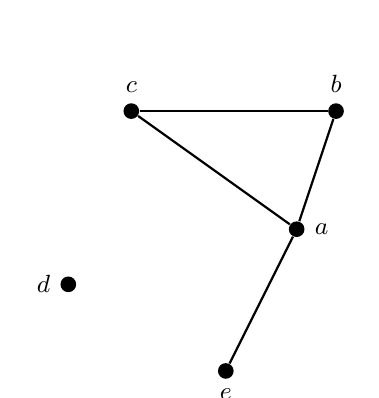
\begin{tikzpicture}[every node/.style={font=\small}]
  \tikzset{dot/.style={circle, fill, inner sep=2pt}}
  \node[dot, label=above:{$c$}] (c) at (-1.6, 1.8) {};
  \node[dot, label=above:{$b$}] (b) at ( 1.0, 1.8) {};
  \node[dot, label=right:{$a$}] (a) at ( 0.5, 0.3) {};
  \node[dot, label=left:{$d$}]  (d) at (-2.4,-0.4) {};
  \node[dot, label=below:{$e$}] (e) at (-0.4,-1.5) {};
  \draw[thick] (c) -- (b);
  \draw[thick] (a) -- (b);
  \draw[thick] (a) -- (c);
  \draw[thick] (a) -- (e);
\end{tikzpicture}
\end{center}

\begin{center}
\renewcommand{\arraystretch}{1.4}
\begin{tabular}{|c|c|c|c|}
\hline
$v$ & $N_G(v)$ & $I_G(v)$ & $\deg_G(v)$ \\
\hline
$a$ & $\{b, c, e\}$ & $\{\{a,b\}, \{a,c\}, \{a,e\}\}$ & $3$ \\
$b$ & $\{a, c\}$    & $\{\{a,b\}, \{b,c\}\}$          & $2$ \\
$c$ & $\{a, b\}$    & $\{\{a,c\}, \{b,c\}\}$          & $2$ \\
$d$ & $\emptyset$   & $\emptyset$                     & $0$ \\
$e$ & $\{a\}$       & $\{\{a,e\}\}$                   & $1$ \\
\hline
\end{tabular}
\end{center}

Sum of degrees: $3+2+2+0+1 = 8 = 2 \cdot 4 = 2 \card{E(G)}$.  This is no
coincidence.

\subsection{The handshaking lemma}

\begin{defbox}
\begin{definition}[Subgraph]
$H \leq G$ iff $V(H) \subseteq V(G)$ and $E(H) \subseteq E(G)$.
\end{definition}
\end{defbox}

\begin{thmbox}
\begin{theorem}[Handshaking lemma]
For every graph $G$,
\[
  2 \cdot \card{E(G)} \;=\; \sum_{v \in V(G)} \deg_G(v).
\]
\end{theorem}
\begin{proof}[Proof by induction on $\card{V(G)}$]
\textit{Base ($n = 0$).}\;
$V(G) = \emptyset$ forces $E(G) = \emptyset$, and both sides equal $0$.

\smallskip
\textit{Step.}\;
Assume the result for $\card{V(G)} = k$ and let $\card{V(G)} = k + 1$.
Pick any $x \in V(G)$ and form $H$ by deleting $x$ and all edges incident
to it:
\[
  V(H) = V(G) \setminus \{x\},\qquad
  E(H) = E(G) \setminus I_G(x) = \{e \in E(G) \mid x \notin e\}.
\]
$H$ is a graph with $\card{V(H)} = k$, so by the inductive hypothesis
$2 \card{E(H)} = \sum_{v \in V(H)} \deg_H(v)$. Two facts about how degrees
change under this deletion:

\smallskip
\emph{(a) Non-neighbours of $x$ keep their degree.}\;
For $v \in V(G) \setminus (N_G(x) \cup \{x\})$, every edge of $G$
containing $v$ also lies in $H$, so $\deg_H(v) = \deg_G(v)$.

\smallskip
\emph{(b) Neighbours of $x$ lose exactly one edge.}\;
For $v \in N_G(x)$, the unique edge $\{v, x\}$ is removed, so
$\deg_H(v) = \deg_G(v) - 1$.

\smallskip
Partitioning $V(G) = N_G(x) \sqcup (V(G) \setminus (N_G(x) \cup \{x\})) \sqcup \{x\}$:
\begin{align*}
  \sum_{v \in V(G)} \deg_G(v)
  &= \sum_{v \in N_G(x)} (\deg_H(v) + 1)
   + \sum_{v \notin N_G(x) \cup \{x\}} \deg_H(v)
   + \deg_G(x) \\
  &= \card{N_G(x)} + \sum_{v \in V(H)} \deg_H(v) + \deg_G(x) \\
  &= \deg_G(x) + 2\card{E(H)} + \deg_G(x)
     \quad \text{(IH; \;$\card{N_G(x)} = \deg_G(x)$)} \\
  &= 2\bigl(\card{I_G(x)} + \card{E(H)}\bigr)
   \;=\; 2 \card{E(G)},
\end{align*}
since $E(G)$ partitions into $I_G(x)$ and $E(H)$.
\end{proof}
\end{thmbox}

\begin{thmbox}
\begin{corollary}[Parity]
The number of odd-degree vertices in any graph is even.
\end{corollary}
\begin{proof}
$\sum_v \deg_G(v) = 2 \card{E(G)}$ is even.  Splitting the sum by parity,
the contribution from even-degree vertices is even, so the contribution
from odd-degree vertices is even too --- and a sum of odd numbers is even
iff there are an even number of summands.
\end{proof}
\end{thmbox}

\begin{notebox}
\begin{example}
For the five-vertex graph above, the odd-degree vertices are $a$ (degree $3$)
and $e$ (degree $1$): two of them, which is even.  \checkmark
\end{example}
\end{notebox}

\begin{notebox}
\begin{remark}[Two ``handshakes'']
The \emph{handshake theorem} (\S\ref{sec:handshake}) and the
\emph{handshaking lemma} (this section) are different results sharing a
metaphor.  Both ultimately depend on the same fact: each edge has two
endpoints, so any quantity counted ``per endpoint'' double-counts edges.
\end{remark}
\end{notebox}

% ════════════════════════════════════════════════════════════════
% EPILOGUE
% ════════════════════════════════════════════════════════════════
\newpage
\section*{Epilogue: the through-line}
\addcontentsline{toc}{section}{Epilogue: the through-line}

The four parts of this document trace a single arc.  Modular arithmetic
gave us our first equivalence relation and the lesson that ``equality up
to'' a relation produces structured quotient sets.  Functions formalised
the language of \emph{maps between sets}.  Cardinality used those maps
--- specifically injections and surjections --- to compare set sizes,
extending counting to the infinite. The applications then deployed all
this machinery: pigeonhole and graph theory both reduce to claims about
how a function's domain and codomain compare.

\begin{notebox}
\begin{remark}[Looking ahead]
The same toolkit drives a great deal of the rest of CS 173 and beyond:
relations and partial orders generalise the equivalence patterns of
Part I, solving linear congruences applies the cancellation theorems of
Part II, and graph theory builds toward connectivity, trees, and graph
isomorphism --- which are themselves ``cardinality of structures'' questions
in disguise.
\end{remark}
\end{notebox}

\end{document}
